\documentclass[11pt]{article}

% ---------- Packages ----------
\usepackage[margin=1in]{geometry}
\usepackage{graphicx}
\usepackage{float}
\usepackage{booktabs}
\usepackage{siunitx}
\usepackage{amsmath}
\usepackage{amssymb}
\usepackage{tikz}
\usetikzlibrary{angles,quotes,arrows.meta,calc}
\usepackage{tcolorbox}
\usepackage{enumitem}
\usepackage{xcolor}
\usepackage{hyperref}
\hypersetup{colorlinks=true, linkcolor=black, urlcolor=blue}

\setlength{\parindent}{0pt}
\setlength{\parskip}{0.6\baselineskip}

\newtcolorbox{finalanswer}{
    colback=white, colframe=black, boxrule=1pt,
    title=Answer, fonttitle=\bfseries, coltitle=black,
    colbacktitle=white
}

\newcommand{\eqlabel}[1]{\textbf{#1}}

\begin{document}

% =========================================================
\begin{titlepage}
    \centering
    \vspace*{2cm}
    {\LARGE \bfseries ENGR 225: Mechanics 1} \\[0.3cm]
    {\Large Homework Coversheet} \\[0.3cm]
    {\large Assoc.\ Prof.\ Clayton Byers} \\[2cm]

    \begin{flushleft}
        \Large
        \textbf{NAME:} Sean Balbale \\[1cm]
        \textbf{DATE:} 18 September 2026 \\[1cm]
        \textbf{ASSIGNMENT:} Homework 1 \\[2cm]
    \end{flushleft}

    \large
    \textbf{Level of involvement of AI, LLMs, or related tools in the completion of this assignment:}

    \vspace{1cm}

    \begin{flushleft}
        \Large
        $\square$ \quad None \\[0.7cm]
        $\blacksquare$ \quad Minor \\[0.7cm]
        $\square$ \quad Major \\[0.7cm]
        $\square$ \quad Extensive \\[1.5cm]
    \end{flushleft}

    \normalsize
    \textit{Mark the box that applies before submitting. Your disclosure does not affect your grade -- it keeps you accountable for the work you are doing.}

\end{titlepage}

\section*{ENGR 225 -- Homework 1 -- Solutions}
% \textbf{Assigned:} 11 Sept 2026 \hfill \textbf{Due:} 18 Sept 2026 (11:59pm on Moodle)

% =========================================================
% PROBLEM 1
% =========================================================
% \clearpage
\section*{Problem 1}

\textbf{Given / Find:} $F_1 = \SI{250}{lb}$ acting $30^\circ$ from the $+y$-axis (tilted toward $+x$); $F_2 = \SI{375}{lb}$ acting $45^\circ$ below the $+x$-axis. Find the magnitude of the resultant $\vec{F}_R = \vec{F}_1+\vec{F}_2$ and its direction $\theta$, measured counterclockwise from the $+x$-axis.

\textbf{Sketch:}
\begin{center}
\begin{tikzpicture}[scale=1.1, >=Stealth]
    \draw[->] (-1,0) -- (3,0) node[right] {$x$};
    \draw[->] (0,-2.2) -- (0,2.6) node[above] {$y$};
    \draw[->, thick, blue] (0,0) -- (0.87,2.30) node[above right] {$F_1=\SI{250}{lb}$};
    \draw[->, thick, red] (0,0) -- (2.65,-2.65) node[below right] {$F_2=\SI{375}{lb}$};
    \draw (0,0.8) arc (90:70:0.8);
    \node at (0.55,0.95) {\footnotesize $30^\circ$};
    \draw (0.9,0) arc (0:-45:0.9);
    \node at (0.95,-0.35) {\footnotesize $45^\circ$};
\end{tikzpicture}
\end{center}

\textbf{Equations \& Solution:}

\eqlabel{Step 1 -- Resolve each force into $x,y$ components.}
Since $F_1$ is measured from the $y$-axis, its horizontal component uses sine and its vertical component uses cosine:
\begin{align*}
    F_{1x} &= F_1 \sin 30^\circ = (250)(0.5) = \SI{125}{lb} \\
    F_{1y} &= F_1 \cos 30^\circ = (250)(0.8660) = \SI{216.5}{lb}
\end{align*}
$F_2$ is measured from the $x$-axis, below it, so its $y$-component is negative:
\begin{align*}
    F_{2x} &= F_2 \cos 45^\circ = (375)(0.7071) = \SI{265.2}{lb} \\
    F_{2y} &= -F_2 \sin 45^\circ = -(375)(0.7071) = \SI{-265.2}{lb}
\end{align*}

\eqlabel{Step 2 -- Sum components.}
\begin{align*}
    R_x &= F_{1x}+F_{2x} = 125 + 265.2 = \SI{390.2}{lb} \\
    R_y &= F_{1y}+F_{2y} = 216.5 - 265.2 = \SI{-48.7}{lb}
\end{align*}

\eqlabel{Step 3 -- Magnitude and direction.}
\begin{align*}
    F_R &= \sqrt{R_x^2+R_y^2} = \sqrt{(390.2)^2+(48.7)^2} = \SI{393}{lb} \\
    \theta' &= \tan^{-1}\!\left(\frac{48.7}{390.2}\right) = 7.11^\circ \quad \text{(below $+x$-axis, since $R_y<0$)}
\end{align*}
Measuring counterclockwise from the $+x$-axis all the way around to the resultant:
\[
    \theta = 360^\circ - 7.11^\circ = 352.9^\circ \approx 353^\circ
\]

\begin{finalanswer}
    $F_R = \SI{393}{lb}$, \quad $\theta = 353^\circ$ measured counterclockwise from the $+x$-axis.
\end{finalanswer}

% =========================================================
% PROBLEM 2
% =========================================================
\clearpage
\section*{Problem 2}

\textbf{Given / Find:} Force $\vec{F}$ acts on frame $ABC$ such that its component along member $AB$ is $\SI{650}{lb}$ (directed $B\to A$) and its component along $BC$ is $\SI{500}{lb}$ (directed $B\to C$), with $\phi = 60^\circ$ at $A$ and $45^\circ$ at $C$. Find $F$ and its direction $\theta$ (measured from the $AB$ axis at $B$).

\textbf{Sketch:}
\begin{center}
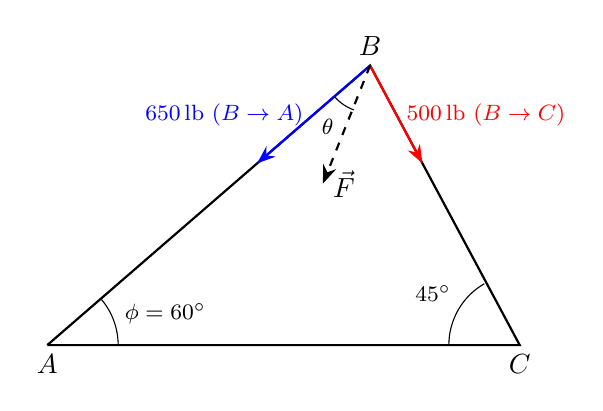
\begin{tikzpicture}[scale=1.0, >=Stealth]
    \coordinate (A) at (0,0);
    \coordinate (C) at (6,0);
    \coordinate (B) at (4.1,3.55); % intersection consistent with 60 and 45 deg
    \draw[thick] (A) -- (B) -- (C) -- (A);
    \draw (A)++(0.9,0) arc (0:40:0.9);
    \node at (1.5,0.4) {\footnotesize $\phi=60^\circ$};
    \draw (C)++(-0.9,0) arc (180:120:0.9);
    \node at (4.9,0.65) {\footnotesize $45^\circ$};
    \draw (B)++(220.87:0.6) arc (220.87:250:0.6);
    \node at ($(B)+(235.5:0.95)$) {\footnotesize $\theta$};
    \node[below] at (A) {$A$};
    \node[below] at (C) {$C$};
    \node[above] at (B) {$B$};
    \draw[->, thick, blue] (B) -- ($(B)!0.35!(A)$) node[midway, left] {\footnotesize $650\,\text{lb (}B\to A\text{)}$};
    \draw[->, thick, red] (B) -- ($(B)!0.35!(C)$) node[midway, right] {\footnotesize $500\,\text{lb (}B\to C\text{)}$};
    \draw[->, thick, dashed] (B) -- ++(-0.6,-1.5) node[right] {$\vec{F}$};
    

\end{tikzpicture}
\end{center}

\textbf{Equations \& Solution:}

\eqlabel{Step 1 -- Interior angle at $B$.} The triangle's angles sum to $180^\circ$:
\[
    \angle B = 180^\circ - \phi - 45^\circ = 180^\circ - 60^\circ - 45^\circ = 75^\circ
\]
This is the angle between the given 650-lb and 500-lb components.

\eqlabel{Step 2 -- Resultant magnitude.}
The 650-lb and 500-lb components add to give $\vec F$:
\begin{align*}
    F &= \sqrt{(650)^2+(500)^2+2(650)(500)\cos 75^\circ} \\
      &= \sqrt{422500+250000+168232} = \sqrt{840732} \\
    F &= \SI{917}{lb}
\end{align*}

\eqlabel{Step 3 -- Direction.}
In the force triangle, the interior angle opposite $F$ is $180^\circ-75^\circ = 105^\circ$. Solving for the angle $\theta$ between $F$ and the 650-lb ($AB$) direction:
\begin{align*}
    \frac{500}{\sin \theta} &= \frac{917}{\sin 105^\circ} \\
    \sin \theta &= \frac{500 \sin 105^\circ}{917} = \frac{482.9}{917} = 0.5267 \\
    \theta &= 31.8^\circ
\end{align*}

\begin{finalanswer}
    $F = \SI{917}{lb}$, \quad $\theta = 31.8^\circ$ from the $AB$ axis.
\end{finalanswer}

% =========================================================
% PROBLEM 3
% =========================================================
\clearpage
\section*{Problem 3}

\textbf{Given / Find:} Two tugboats pull a barge: $\vec{F}_A = \SI{2}{kN}$ at $30^\circ$ above the $+x$-axis, and $\vec{F}_B$ (unknown) below the $x$-axis at angle $\theta$. The resultant is $\SI{3}{kN}$ directed along the $+x$-axis. Find $F_B$ and $\theta$.

\textbf{Sketch:}
\begin{center}
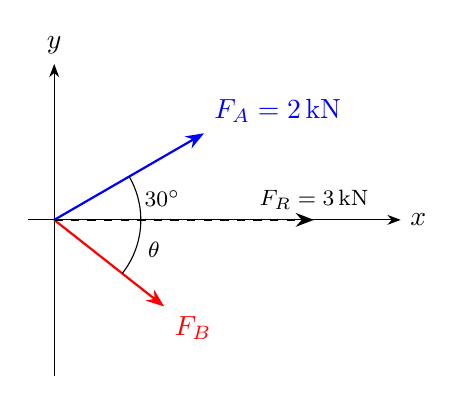
\begin{tikzpicture}[scale=1.1,>=Stealth]
    \draw[->] (-0.3,0) -- (4,0) node[right] {$x$};
    \draw[->] (0,-1.8) -- (0,1.8) node[above] {$y$};
    \draw[->,thick,blue] (0,0) -- (1.73,1.0) node[above right] {$F_A = \SI{2}{kN}$};
    \draw[->,thick,red] (0,0) -- (1.27,-1.0) node[below right] {$F_B$};
    \draw[->,thick,dashed] (0,0) -- (3,0) node[above] {\footnotesize $F_R = \SI{3}{kN}$};
    \draw (1,0.0) arc (0:30:1);
    \node at (1.25,0.25) {\footnotesize $30^\circ$};
    \draw (1.0,0) arc (0:-38:1.0);
    \node at (1.15,-0.35) {\footnotesize $\theta$};
\end{tikzpicture}
\end{center}

\textbf{Equations \& Solution:}

\eqlabel{Step 1 -- Components of $F_A$.}
\begin{align*}
    F_{Ax} &= 2\cos 30^\circ = \SI{1.732}{kN} \\
    F_{Ay} &= 2\sin 30^\circ = \SI{1.000}{kN}
\end{align*}

\eqlabel{Step 2 -- Require the resultant equal $\SI{3}{kN}$ along $+x$ with zero $y$-component.}
\begin{align*}
    F_{Ax}+F_{Bx} &= 3 \quad\Rightarrow\quad F_{Bx} = 3-1.732 = \SI{1.268}{kN} \\
    F_{Ay}+F_{By} &= 0 \quad\Rightarrow\quad F_{By} = -1.000\,\text{kN (below $x$-axis)}
\end{align*}

\eqlabel{Step 3 -- Magnitude and direction of $F_B$.}
\begin{align*}
    F_B &= \sqrt{(1.268)^2+(1.000)^2} = \sqrt{1.608+1.000} = \SI{1.61}{kN} \\
    \theta &= \tan^{-1}\!\left(\frac{1.000}{1.268}\right) = 38.2^\circ \ \text{below the $+x$-axis}
\end{align*}

\begin{finalanswer}
    $F_B = \SI{1.61}{kN}$, \quad $\theta = 38.2^\circ$ below the $+x$-axis.
\end{finalanswer}

% =========================================================
% PROBLEM 4
% =========================================================
\clearpage
\section*{Problem 4}

\textbf{Given / Find:} $F_1 = \SI{200}{N}$ acts horizontally. The $y$-axis is $45^\circ$ from horizontal (from $F_1$), and the figure's $x$-axis (the dashed reference line) is $90^\circ$ from the $y$-axis --- i.e.\ also $45^\circ$ from $F_1$, on the other side, as shown. $F_2 = \SI{150}{N}$ acts $30^\circ$ from this $x$-axis reference line. Find the resultant magnitude and its direction $\theta$, measured counterclockwise from the positive $x$-axis defined in the figure.

\textbf{Sketch:}
\begin{center}
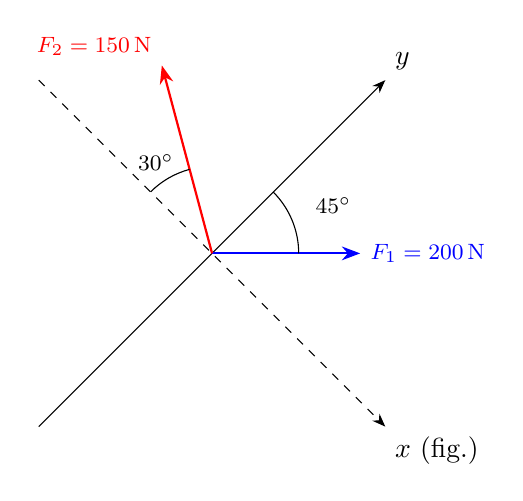
\begin{tikzpicture}[scale=1.1,>=Stealth]
    \draw[->] (-2,-2) -- (2,2) node[above right] {$y$};
    \draw[->,dashed] (-2,2) -- (2,-2) node[below right] {$x$ (fig.)};
    \draw[->,thick,blue] (0,0) -- (1.71,0) node[right] {\footnotesize $F_1=\SI{200}{N}$};
    \draw[->,thick,red] (0,0) -- (-0.58,2.17) node[above left] {\footnotesize $F_2=\SI{150}{N}$};
    \node at (1.4,0.55) {\footnotesize $45^\circ$};
    \draw (1.0,0) arc (0:45.0:1.0);
    \node at (-0.65,1.05) {\footnotesize $30^\circ$};
    \draw (-0.26,0.97) arc (105:135:1.0);
\end{tikzpicture}
\end{center}

\textbf{Equations \& Solution:}

\eqlabel{Step 1 -- Locate each force relative to the figure's $x$-axis.}
$F_1$ is horizontal, with the $y$-axis $45^\circ$ above it; since the figure's $x$-axis is $90^\circ$ from $y$, it falls $45^\circ$ below $F_1$ on the other side, so $F_1$ makes a $45^\circ$ angle with the figure's $x$-axis. $F_2$ is $30^\circ$ from the same $x$-axis line, on the side toward the $y$-axis --- i.e.\ $30^\circ$ short of the line's upper ray --- so measured from the figure's positive $x$-axis it lies at $180^\circ - 30^\circ = 150^\circ$.

\eqlabel{Step 2 -- Components (in the figure's $x$--$y$ system).}
\begin{align*}
    F_{1x} &= 200\cos 45^\circ = \SI{141.4}{N} & F_{1y} &= 200 \sin 45^\circ = \SI{141.4}{N} \\
    F_{2x} &= 150 \cos 150^\circ = \SI{-129.9}{N} & F_{2y} &= 150 \sin 150^\circ = \SI{75.0}{N}
\end{align*}

\eqlabel{Step 3 -- Sum and resolve.}
\begin{align*}
    R_x &= 141.4 - 129.9 = \SI{11.5}{N} \\
    R_y &= 141.4 + 75.0 = \SI{216.4}{N} \\
    F_R &= \sqrt{(11.5)^2+(216.4)^2} = \SI{217}{N} \\
    \theta &= \tan^{-1}\!\left(\frac{216.4}{11.5}\right) = 87.0^\circ
\end{align*}

\begin{finalanswer}
    $F_R = \SI{217}{N}$, \quad $\theta = 87.0^\circ$ ccw from the figure's $+x$-axis.
\end{finalanswer}

% =========================================================
% PROBLEM 5
% =========================================================
\clearpage
\section*{Problem 5}

\textbf{Given / Find:} A bracket carries $\SI{14}{kN}$ at $30^\circ$ above the $-x$-axis and $\SI{8}{kN}$ along $+x$, plus a variable force $\vec{F}$ acting along a fixed $45^\circ$ line. Find $F$ so that the resultant is as small as possible, and find that minimum resultant $F_R$.

\textbf{Sketch:}
\begin{center}
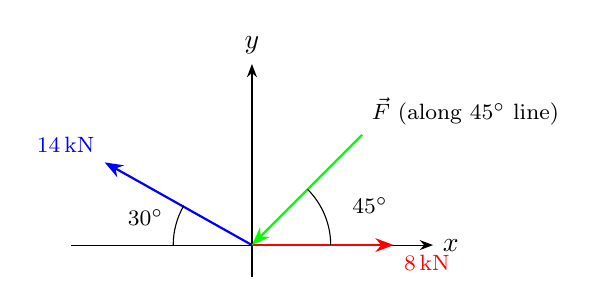
\begin{tikzpicture}[scale=1.0,>=Stealth]
    \draw[->] (-2.3,0) -- (2.3,0) node[right] {$x$};
    \draw[->] (0,-0.4) -- (0,2.3) node[above] {$y$};
    \draw[->,thick,blue] (0,0) -- (-1.87,1.05) node[above left] {\footnotesize $\SI{14}{kN}$};
    \draw[->,thick,red] (0,0) -- (1.8,0) node[below right] {\footnotesize $\SI{8}{kN}$};
    \draw[->,thick,green] (1.4,1.4) -- (0,0);
    \node[above right] at (1.4,1.4) {\footnotesize $\vec{F}$ (along $45^\circ$ line)};
    \node at (-1.35,0.35) {\footnotesize $30^\circ$};
    \draw (-0.866,0.5) arc (150:180:1.0);
    \node at (1.5,0.50) {\footnotesize $45^\circ$};
    \draw (1.0,0) arc (0:45.0:1.0);
\end{tikzpicture}
\end{center}

\textbf{Equations \& Solution:}

\eqlabel{Step 1 -- Sum the two fixed forces.}
\begin{align*}
    S_x &= 14\cos 150^\circ + 8 = -12.12+8 = \SI{-4.12}{kN} \\
    S_y &= 14 \sin 150^\circ = \SI{7.00}{kN}
\end{align*}

\eqlabel{Step 2 -- Add the variable force $F$ along the $45^\circ$ line.}
\[
    R_x = S_x+F\cos 45^\circ, \qquad R_y = S_y+F\sin 45^\circ
\]
\[
    F_R^2 = (S_x+F\cos 45^\circ)^2+(S_y+F\sin 45^\circ)^2
\]

\eqlabel{Step 3 -- Minimize: set $\dfrac{d(F_R^2)}{dF}=0$.}
\[
    \cos45^\circ (S_x+F\cos45^\circ)+\sin45^\circ(S_y+F\sin45^\circ)=0
\]
Since $\cos^2 45^\circ+\sin^2 45^\circ = 1$:
\[
    F = -\left(S_x\cos45^\circ+S_y\sin45^\circ\right) = -\big[(-4.12)(0.7071)+(7.00)(0.7071)\big] = \SI{-2.03}{kN}
\]
\[
    F = \SI{2.03}{kN}
\]

\eqlabel{Step 4 -- Compute the resulting minimum $F_R$.}
\begin{align*}
    R_x &= -4.12+(-2.03)(0.7071) = \SI{-5.56}{kN} \\
    R_y &= 7.00+(-2.03)(0.7071) = \SI{5.56}{kN} \\
    F_R &= \sqrt{(5.56)^2+(5.56)^2} = \SI{7.87}{kN}
\end{align*}

\begin{finalanswer}
    $F = \SI{2.03}{kN}$ (directed opposite the drawn $45^\circ$ ray), giving a minimum resultant $F_R = \SI{7.87}{kN}$.
\end{finalanswer}

% =========================================================
% PROBLEM 6
% =========================================================
\clearpage
\section*{Problem 6}

\textbf{Given / Find:} $F_1 = \SI{450}{N}$ lies in the $y$--$z$ plane, defined by a 3-4-5 triangle ($F_{1x}=0$). $F_2=\SI{525}{N}$ has coordinate direction angles $\alpha=45^\circ$ (from $x$), $\beta=120^\circ$ (from $y$), $\gamma=60^\circ$ (from $z$). Find the magnitude and coordinate direction angles of the resultant, and sketch it.

\textbf{Sketch:}
\begin{center}
\begin{tikzpicture}[scale=1.0,>=Stealth,
        x={(-0.52cm,-0.30cm)}, y={(0.78cm,-0.14cm)}, z={(0cm,1cm)}]
    % --- Axes: z up (full length), x foreshortened toward the viewer,
    %     y only lightly foreshortened (closer to the page plane) ---
    \draw[->] (0,0,0) -- (3.5,0,0) node[below left] {$x$};
    \draw[->] (0,0,0) -- (0,3,0) node[right] {$y$};
    \draw[->] (0,0,0) -- (0,0,3.2) node[above] {$z$};
    % --- F1 = 450 N, entirely in the y-z plane (3-4-5 triangle: Fy=+3/5, Fz=-4/5) ---
    \draw[->,thick,blue] (0,0,0) -- (0,1.8,-2.4) node[below] {\footnotesize $F_1=\SI{450}{N}$};
    % --- F2 = 525 N, direction angles alpha=45 (x), beta=120 (y), gamma=60 (z) ---
    \draw[->,thick,red] (0,0,0) -- (2.48,-1.75,1.75) node[above left] {\footnotesize $F_2=\SI{525}{N}$};
    % --- Resultant ---
    \draw[->,thick,dashed] (0,0,0) -- (2.48,0.05,-0.65) node[below left] {\footnotesize $F_R=\SI{384}{N}$};
    % --- Angle arcs for F2, drawn at the true on-page ray angles (z=90, F2=154.7, x=210, y=-10.2) ---
    \begin{scope}[x={(1cm,0cm)}, y={(0cm,1cm)}]
        \draw (90:0.9) arc (90:154.7:0.9);
        \node at (122.4:1.15) {\footnotesize $60^\circ$};
        \draw (154.7:0.6) arc (154.7:210:0.6);
        \node at (182.4:0.9) {\footnotesize $45^\circ$};
        \draw (-10.2:1.3) arc (-10.2:154.7:1.3);
        \node at (72.3:1.6) {\footnotesize $120^\circ$};
    \end{scope}
\end{tikzpicture}
\end{center}

\textbf{Equations \& Solution:}

\eqlabel{Step 1 -- Components of $F_1$ (3-4-5 triangle, in the $y$-$z$ plane).}
\begin{align*}
    F_{1x} &= 0 \\
    F_{1y} &= 450\left(\tfrac{3}{5}\right) = \SI{270}{N} \\
    F_{1z} &= -450\left(\tfrac{4}{5}\right) = \SI{-360}{N}
\end{align*}

\eqlabel{Step 2 -- Components of $F_2$ (direction cosines).}
\begin{align*}
    F_{2x} &= 525\cos45^\circ = \SI{371.2}{N} \\
    F_{2y} &= 525\cos120^\circ = \SI{-262.5}{N} \\
    F_{2z} &= 525\cos60^\circ = \SI{262.5}{N}
\end{align*}
\emph{Check:} $\cos^2 45^\circ+\cos^2120^\circ+\cos^260^\circ = 0.5+0.25+0.25=1$ \checkmark

\eqlabel{Step 3 -- Sum components.}
\begin{align*}
    R_x &= 0+371.2 = \SI{371.2}{N} \\
    R_y &= 270-262.5 = \SI{7.5}{N} \\
    R_z &= -360+262.5 = \SI{-97.5}{N}
\end{align*}

\eqlabel{Step 4 -- Magnitude and coordinate direction angles.}
\begin{align*}
    F_R &= \sqrt{(371.2)^2+(7.5)^2+(-97.5)^2} = \sqrt{147{,}373} = \SI{384}{N} \\
    \alpha &= \cos^{-1}\!\left(\frac{371.2}{384}\right) = 14.8^\circ \\
    \beta &= \cos^{-1}\!\left(\frac{7.5}{384}\right) = 88.9^\circ \\
    \gamma &= \cos^{-1}\!\left(\frac{-97.5}{384}\right) = 105^\circ
\end{align*}

\begin{finalanswer}
    $F_R = \SI{384}{N}$, \quad $\alpha = 14.8^\circ$, \quad $\beta = 88.9^\circ$, \quad $\gamma = 105^\circ$.
\end{finalanswer}

% =========================================================
% PROBLEM 7
% =========================================================
\clearpage
\section*{Problem 7}

\textbf{Given / Find:} A plate is suspended from point $A$ by three cables to corners $B$, $C$, $D$, with tensions $F_{BA}=\SI{350}{lb}$, $F_{CA}=\SI{500}{lb}$, $F_{DA}=\SI{400}{lb}$. $A$ is $\SI{14}{ft}$ above the plate. Using the in-plane offsets given in the figure, express each cable tension as a Cartesian vector.

\textbf{Sketch:}
\begin{center}
\begin{tikzpicture}[scale=0.85,>=Stealth]
    % Screen coords = x*(-0.55,-0.30) + y*(0.45,-0.10) + z*(0,0.5), matching the
    % solved geometry A=(0,0,14), B=(5,-6,0), C=(-3,-3,0), D=(2,6,0) [ft]
    \coordinate (O) at (0,0);      % point on the plate directly below A
    \coordinate (A) at (0,7);
    \coordinate (B) at (-5.45,-0.9);   % corner: (5,-6,0)
    \coordinate (C) at (-0.55,1.4);     % on the back edge: (-3,-3,0)
    \coordinate (D) at (1.6,-1.2);     % on the right edge: (2,6,0)
    \coordinate (P2) at (-0.05,-2.1);  % corner: (5,6,0)   [front-right, no cable]
    \coordinate (P3) at (4.35,0.3);    % corner: (-3,6,0)  [back-right, no cable]
    \coordinate (P4) at (-1.05,1.5);   % corner: (-3,-6,0) [back-left, no cable]
    % Coordinate axes, from the point directly below A
    \draw[->] (O) -- ++(-3.85,-2.10) node[below] {$x$};
    \draw[->] (O) -- ++(3.15,-0.70) node[below right] {$y$};
    \draw[->] (O) -- (0,8) node[above] {$z$};
    % Plate outline (transparent, dotted) -- a true rectangle; C and D fall on its edges
    \draw[dotted] (B) -- (P2) -- (P3) -- (P4) -- cycle;
    % Points
    \fill (A) circle (2pt) node[above] {$A$};
    \fill (B) circle (2pt) node[left] {$B$};
    \fill (C) circle (2pt) node[above right] {$C$};
    \fill (D) circle (2pt) node[below right] {$D$};
    % Height dimension
    \draw[dashed] (O) -- (A);
    \node[left] at (0,3.5) {\footnotesize $14$ ft};
    % Cables (pulling each corner up toward A)
    \draw[thick,blue,->] (B) -- (A) node[midway,left] {\footnotesize $F_{BA}=350\,\text{lb}$};
    \draw[thick,red,->] (C) -- (A) node[midway,above right] {\footnotesize $F_{CA}=500\,\text{lb}$};
    \draw[thick,green!50!black,->] (D) -- (A) node[midway,right] {\footnotesize $F_{DA}=400\,\text{lb}$};
\end{tikzpicture}
\end{center}

\textbf{Equations \& Solution:}

\eqlabel{Step 1 -- Coordinates.}
Placing the ground point directly beneath $A$ at the origin, with $A$ at height $\SI{14}{ft}$, the given in-plane offsets locate the corners at:
\[
    A=(0,0,14),\quad B=(5,-6,0),\quad C=(-3,-3,0),\quad D=(2,6,0)\ \text{[ft]}
\]

\eqlabel{Step 2 -- Position vectors and cable lengths.}
\begin{align*}
    \vec{r}_{BA} &= A-B = (-5,\,6,\,14)\,\text{ft}, & L_{BA} &= \sqrt{5^2+6^2+14^2} = \SI{16.03}{ft} \\
    \vec{r}_{CA} &= A-C = (3,\,3,\,14)\,\text{ft}, & L_{CA} &= \sqrt{3^2+3^2+14^2} = \SI{14.63}{ft} \\
    \vec{r}_{DA} &= A-D = (-2,\,-6,\,14)\,\text{ft}, & L_{DA} &= \sqrt{2^2+6^2+14^2} = \SI{15.36}{ft}
\end{align*}

\eqlabel{Step 3 -- Unit vectors and force vectors ($\vec{F}=F\cdot \hat u = F\,\vec r/L$).}
\begin{align*}
    \vec{F}_{BA} &= 350\cdot\frac{(-5,6,14)}{16.03} = -109\hat i+131\hat j+306\hat k\ \text{lb} \\
    \vec{F}_{CA} &= 500\cdot\frac{(3,3,14)}{14.63} = 103\hat i+103\hat j+479\hat k\ \text{lb} \\
    \vec{F}_{DA} &= 400\cdot\frac{(-2,-6,14)}{15.36} = -52.1\hat i-156\hat j+365\hat k\ \text{lb}
\end{align*}

\begin{finalanswer}
    $\vec{F}_{BA} = -109\hat i+131\hat j+306\hat k\ \text{lb}$ \\
    $\vec{F}_{CA} = 103\hat i+103\hat j+479\hat k\ \text{lb}$ \\
    $\vec{F}_{DA} = -52.1\hat i-156\hat j+365\hat k\ \text{lb}$
\end{finalanswer}

% =========================================================
% PROBLEM 8
% =========================================================
\clearpage
\section*{Problem 8}

\textbf{Given / Find:} Flagpole $OA$ ($O$ at the base, $A$ at the top) is guyed by cables $AB$ and $AC$ anchored to a wall. Using the dimensions shown, find the angles $\theta$ (between $OA$ and $AB$) and $\phi$ (between $OA$ and $AC$).

\textbf{Sketch:}
\begin{center}
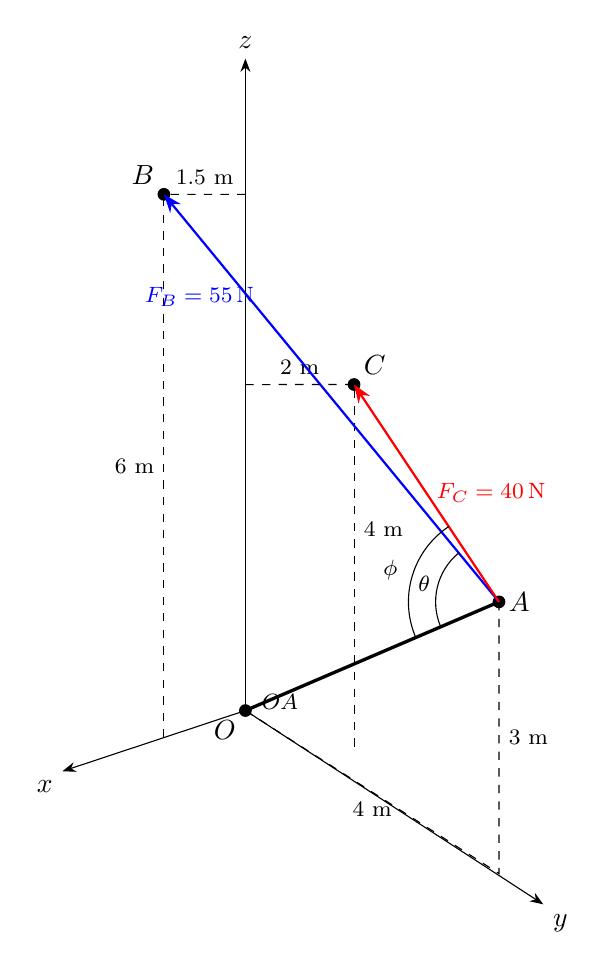
\begin{tikzpicture}[scale=1.15,>=Stealth]
    % Screen coords = x*(0.7,-0.45) + y*(-0.6,-0.2) + z*(0,1), matching the
    % solved geometry O=(0,0,0), A=(4,0,3), B=(0,1.5,6), C=(0,2,4) [m]
    \coordinate (O) at (0,0);
    \coordinate (A) at (2.8,1.2);
    \coordinate (B) at (-0.9,5.7);
    \coordinate (C) at (1.2,3.6);       % mirrored to the other side of the z-axis from B
    \coordinate (Abase) at (2.8,-1.8);  % (4,0,0)
    \coordinate (Bbase) at (-0.9,-0.3); % (0,1.5,0)
    \coordinate (Cbase) at (1.2,-0.4);  % (0,2,0), mirrored to match (C)
    % Axes (labels swapped to match the reference figure, and lengthened)
    \draw[->] (O) -- (0,7.2) node[above] {$z$};
    \draw[->] (O) -- ++(3.29,-2.14) node[below right] {$y$};
    \draw[->] (O) -- ++(-2.02,-0.67) node[below left] {$x$};
    % Height / wall-offset dimensions
    \draw[dashed] (O) -- (Abase) -- (A);
    \node[below] at ($(O)!0.5!(Abase)$) {\footnotesize $4$ m};
    \node[right] at ($(Abase)!0.5!(A)$) {\footnotesize $3$ m};
    \draw[dashed] (Bbase) -- (B);
    \node[left] at ($(Bbase)!0.5!(B)$) {\footnotesize $6$ m};
    \draw[dashed] (0,5.7) -- (B);
    \node[above] at ($(0,5.7)!0.5!(B)$) {\footnotesize $1.5$ m};
    \draw[dashed] (Cbase) -- (C);
    \node[right] at ($(Cbase)!0.6!(C)$) {\footnotesize $4$ m};
    \draw[dashed] (0,3.6) -- (C);
    \node[above] at ($(0,3.6)!0.5!(C)$) {\footnotesize $2$ m};
    % Points
    \fill (O) circle (2pt) node[below left] {$O$};
    \fill (A) circle (2pt) node[right] {$A$};
    \fill (B) circle (2pt) node[above left] {$B$};
    \fill (C) circle (2pt) node[above right] {$C$};
    % Flagpole and cables
    \draw[very thick] (O) -- (A) node[pos=0.25,below left] {\footnotesize $OA$};
    \draw[thick,blue,->] (A) -- (B) node[pos=0.7,above left] {\footnotesize $F_B=\SI{55}{N}$};
    \draw[thick,red,->] (A) -- (C) node[midway,right] {\footnotesize $F_C=\SI{40}{N}$};
    % Angles at A between AO and each cable (on-screen rays: AO=203.2, AB=129.4, AC=123.7)
    \draw ($(A)+(203.2:0.7)$) arc (203.2:129.4:0.7);
    \node at ($(A)+(166.3:0.85)$) {\footnotesize $\theta$};
    \draw ($(A)+(203.2:1.0)$) arc (203.2:123.7:1.0);
    \node at ($(A)+(163.5:1.25)$) {\footnotesize $\phi$};
\end{tikzpicture}
\end{center}

\textbf{Equations \& Solution:}

\eqlabel{Step 1 -- Coordinates from the given dimensions.}

\[
    O=(0,0,0),\quad A=(0,4,3),\quad B=(1.5,0,6),\quad C=(-2,0,4)\ \text{[m]}
\]

\eqlabel{Step 2 -- Vectors from vertex $A$.}
\begin{align*}
    \vec{AO} &= O-A = (0,\,-4,\,-3)\,\text{m}, & |\vec{AO}| &= \sqrt{4^2+3^2} = \SI{5.00}{m} \\
    \vec{AB} &= B-A = (1.5,\,-4,\,3)\,\text{m}, & |\vec{AB}| &= \sqrt{1.5^2+4^2+3^2} = \SI{5.22}{m} \\
    \vec{AC} &= C-A = (-2,\,-4,\,1)\,\text{m}, & |\vec{AC}| &= \sqrt{2^2+4^2+1^2} = \SI{4.58}{m}
\end{align*}

\eqlabel{Step 3 -- Angle $\theta$ between $AO$ and $AB$.}
\begin{align*}
    \vec{AO}\cdot\vec{AB} &= (0)(1.5)+(-4)(-4)+(-3)(3) = 0+16-9 = 7 \\
    \cos\theta &= \frac{7}{(5.00)(5.22)} = 0.2682 \\
    \theta &= 74.4^\circ
\end{align*}

\eqlabel{Step 4 -- Angle $\phi$ between $AO$ and $AC$.}
\begin{align*}
    \vec{AO}\cdot\vec{AC} &= (0)(-2)+(-4)(-4)+(-3)(1) = 0+16-3 = 13 \\
    \cos\phi &= \frac{13}{(5.00)(4.58)} = 0.5674 \\
    \phi &= 55.4^\circ
\end{align*}

\begin{finalanswer}
    $\theta = 74.4^\circ$, \quad $\phi = 55.4^\circ$.
\end{finalanswer}

\end{document}